\documentclass[a4paper,11pt]{article}
\usepackage[margin=2cm]{geometry}
\usepackage[utf8]{inputenc}
\usepackage[french]{babel} % to write in french
\usepackage[final]{pdfpages} % include pdf files
\usepackage{enumitem}
\usepackage{eurosym}
\usepackage{amsmath}

\begin{document}

\begin{titlepage}
\begin{center}
	{\sc Université libre de Bruxelles}\\
	Faculté des Sciences\\
	Département d'Informatique
	\vfill{}\vfill{}

	{\Huge \par}{\Huge Decision Engineering}{\Huge \par}
	{\Huge \par}{\huge Cloud service providers comparison}{\Huge \par}

	{\huge \par}{\Large Xavier Barthel, }
				{\Large Victor Carakehian}{\huge \par}
	
	\vfill{}
	
\includegraphics{img/ulb_symbol.pdf}

	\vfill{}\vfill{}
	Année académique 2014~--~2015
\end{center}
\end{titlepage}

\section{Introduction}
This project is about choosing an alternative amongst multiple other ones. The process of choosing an alternative is simple when it is done on the basis of a single criterion. However, most of the time a decision involves more than one criterion for decision-making process and the complex decision problems can not be resolved on the basis of unidimensional approaches. The difficulty resides in evaluating alternatives taking in account criteria. Those criteria are often conflicting and do not use the same units to quantify them.\\

In order to establish a ranking of the alternatives, Multi-Criteria Decision Analysis (MCDA) has lead to the creation of ranking methods such as PROMETHEE, ELECTRE or AHP. The purpose of MCDA is to help decision makers by modeling and representing his preferences. In this project, we used an implementation of the PROMETHEE method, made available by the D-Sight Software Company, to perform a market analysis and comparison of cloud service providers. We will define each criterion held for the comparison, give the precise way we measure it and discuss the weight we gave to it. We will then analyse the results provided by the D-Sight's platform.\\ % TODO: MCDA provides a set of criteria aggregation methodologies.


\section{Context}
This project is about trying to find the best fitting cloud solution for the Railnova\footnote{https://www.railnova.eu/} company. Since the number of cloud providers and their services is always growing, it becomes more and more difficult over time to make a wise choice without a good study. As a provider of telematics solutions for the railway world, Railnova has multiple needs of computation, data storage and connectivity capabilities. To find a good solution, we based our researches on the present solution delivered by OVH to Railnova which consist of two dedicated servers:
\begin{enumerate}
  \item 32 cores with 128Go of RAM and 256 Go SSD of data storage;
  \item 16 cores with 64Go of RAM and 2To of data storage.
\end{enumerate}
Those two servers are entirely managed by Railnova developers and used for two main activities:
\begin{enumerate}
  \item hosting a database containing all the data exploited in production and running the websites in production;
  \item hosting a database containing all the telematics messages ever sent by the embedded devices and applications to receive and process all those messages (a switched on device send one message each 40 seconds and there is 200 devices in production).
\end{enumerate}
From those specifications, we selected the providers' solution fitting it and made comparisons on them.\\

\section{Alternatives}
To evaluate cloud services, the situation is more complex than it appears because the market is full of meaningless (catchy) keywords and the companies are doing there best to complicate the comparisons. Mainly, the different types of cloud computing services can be referred to Software as a Service (SaaS), Infrastructure as a Service (IaaS) or Platform as a Service (PaaS). Taking in account the needs of the decision maker, we will only consider IaaS et PaaS solutions in the following report.\\

\begin{description}[parsep=10pt,labelindent=\parindent]
  \item[IaaS] is an abstraction of the hardware for customers which need to work with virtual machines that they configure themselves.
  \item[PaaS] is a type service which can be seen as an upper layer over IaaS solutions, consisting in a set of tools and libraries designed to make coding and deploying applications easier.
\end{description}

The advantage of PaaS solutions is about being fully focused on the development of the hosted application. Thanks to this kind of service, testing and deployment are automated. The same comes for the scalability of the application which is made easy by the simple use of a web interface and/or a command line. This kind of service can also be easily linked to use-case dedicated services as database instances.\\

For the IaaS, the advantage is about control on the infrastructure, the resources (RAM, CPU, Bandwidth, ...) are shared and virtual machines are running on it. IaaS can be seen as the basic form of cloud on which PaaS is stacked. The trade-off is clear, either you take care of the running environments of your application which means having \emph{control} over the environment, either you pay someone to do it for you and you improve your \emph{productivity}.\\

After some research, we can see that the situation is far from being as simple as a binary classification for hosting application. As an example, the Managed Virtual Machines of the Google App Engine solution which is of the PaaS type but it's purpose is to manage virtual machines of IaaS solution.\\

It is then asked to rank solutions of the two types while keeping in mind the current solution used is an IaaS. To do so, four IaaS providers (RackSpace, Amazon AWS, LeaseWeb, OVH) and 2 PaaS providers (Google App Engine, Heroku) are constituting the alternatives set.

\section{Criteria}

Several criteria are proposed in the literature for the evaluation of cloud services. The criteria which are used in this work has been chosen among the ones mentioned in several works about Quality of Service (QoS) based selection based on the company's preferences.
Those criteria are defined as:

\begin{description}[parsep=10pt,listparindent=\parindent,labelindent=\parindent,font=$\bullet$\ ]
  \item[Availability:] The average amount of time during which the service is accessible and operational.
    \par \emph{Note:} A very common way to evaluate the availability is to use the downtime per year.
    \par \emph{Measurement:} This criterion is expressed as a percentage of the downtime. The used formula is $\frac{t_{st}-t_{dt}}{t_{st}}*100$, where $t_{st}$ is the total service time and $t_{dt}$ is the total down-time. The value of this criterion must be maximized and a usual preference function is used.

  \item[Service efficiency:] How well does a provider responds and implements a given request emitted by the client.
     \par \emph{Note:} When a client request new VM or new database instances, the time spent to accomplish that request has an impact on the client productivity.
    \par \emph{Measurement:} The time (in minute) spent between the costumer request emission and its implementation by the provider. This value must be minimized and a U-shape preference function is used with an indifference threshold of 10 minutes.

  \item[Cost:] The fee that the costumer must pay by using the given service.
    \par \emph{Note:} There is several type of pricing scheme and even a same provider offers different solutions which are suitable for the consumer requirements. For the same price, services can offer different amount of data storage, RAM, number of CPU cores, CPU frequency and bandwidth capacity. In addition, we must take in consideration the cost of what part of the offer price is dedicated to the human management price. Indeed, a solution costing 100\euro{} with a 10\% part dedicated to human cost is more likely to please Railnova than a solution costing 100\euro{} with a 80\% part dedicated to human cost. Because it supposes that the rest of the price is dedicated to the actual hardware and technology provided. This \og human \fg{} cost must be isolated from the price of the solution.
    \par \emph{Measurement:} The cost is defined by the price of the solution made available by the provider. This value must be minimized and a linear preference function is used with an indifference threshold of 250\euro{} and a preference threshold of 500\euro.

  \item[Reputation:] The reputation is the opinion of the user toward the provider.
    \par \emph{Note:} The reputation of a service provider has an impact on the productivity. An employee working with a solution in which he does not have motivation to work with may give rise to additional costs. A provider got extra score when giving donation to open source and for innovation.
    \par \emph{Measurement:} This is expressed as a scale from 1 to 5. This value must maximized and a usual preference function is used.
    
  \item[Portability:] The ability to easily port a solution to another service provider.
    \par \emph{Note:} This criteria is complex to evaluate. Thus, to tackle this criteria, we have decided to express it as the capacity of reimplementing the application on a server owned by the customer. Mainly this is expressed as the availability of open-source API, framework, library and standard software compliance.
    \par \emph{Measurement:} As a quality measurement, this is expressed as a scale from 1 to 5. This value must maximized and a usual preference function is used.

  \item[Usability:] The extent to which the service is easy to use and comprehend.
    \par \emph{Note:} Good documentation is useful when trying new features or in case of failure. A easy to understand and easy to use solution is also a contextual criterion, i.e. the migration, of the current solution, difficulty is taken in account while giving a score.
    \par \emph{Measurement:} A scale from 1 to 3 is used to express the subjective perception. This value must maximized and a usual preference function is used.

  \item[Reliability:] The reliability is the extent to which the provider meets the performance level promised.
    \par \emph{Note:} Reliability is mainly assured by using systems which are redundantly designed, not dependent on the geographical and physical position and use robust software fail-over to withstand disruption.
    \par \emph{Measurement:} The criteria his highly dependent on the policy of the provider, which may include business continuity plan in case of major disaster as much as he can cover hardware failure scenario. Then, this criteria is evaluated with a scale from 1 to 3. This value must maximized and a usual preference function is used.

  \item[Security:] The extent to which the provider can assure the protection of data exchange and the access control.
    \par \emph{Note:} There are multiple mechanisms to achieve the protection of the application. For example, encryption of data transfer must be assure for intern and extern movements. Another example is that, the security of the application must be guaranteed even against users which are executing on the same machine. Hardware and physical security must be assure too. 
    \par \emph{Measurement:} First, we will determine which are the common security mechanisms implemented by every cloud solutions. Then, we list and sum up all the extra security measures implemented by each cloud service provider, and substract the obtained value by the common factor. This value must be maximized and a U-shape preference function is used with an indifference threshold of 2.

  \item[Data Integrity:] The extent to which the client is confident in the data preservation capacity of the provider.
    \par \emph{Note:} It is important that the provider guaranties how the data are preserved. It must also ensure that they remain accurate.
    \par \emph{Measurement:} A scale from 1 (no backup) to 10 (multiple backups with mechanisms that verify the integrity of those backup for free). The values in-between will be regulated by the price of the mechanisms that verify integrity. This value must maximized and a U-shape preference function is used with an indifference threshold of 3.

  \item[Scalability:] Ability and cost to change the size of the resources used.
    \par \emph{Note:} As a growing company, the client is interested about finding a solution that has a good capacity to respond to bigger computation needs. The evolution of the cost given the size of resources used is often non-linear so it must be taken in account.
    \par \emph{Measurement:} The value is computed by comparison of the price of 10 times the present resources following a linear growth and the real price of the solution for 10 times the present resources. This value must be minimized and a linear preference function is used with an indifference threshold of 500\euro{} and a preference threshold of 2000\euro{}.

\end{description}

The final evaluation table is given in figure~\ref{fig:eval}.

\begin{figure}[h]
  \center
  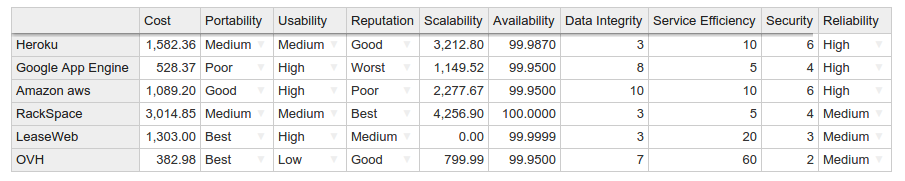
\includegraphics[width=\textwidth]{img/Result/evaluation.png}
  \caption{Evaluation of the alternatives for each criteria.}
  \label{fig:eval}
\end{figure}

\subsection{Weights}
The weights are expressing the decision maker priority in the matter of ranking cloud services. Of course, the cost to acquire a service is one of the most important criteria, which must be minimized. Secondly, the usability and the portability are the second most important criteria, this is explained by the impact on the productivity it could induce. Thirdly, data integrity is important because of the Railnova's field of activity, they need to keep in safety the telematics' data collected over time. And then, comes the last batch of common features. Those weights can be seen as the current weight in the figure~\ref{fig:stab}.

\section{Analysis}
\subsection{Ranking}
The final ranking is given in figure~\ref{fig:ranking}. We can see that the OVH alternative is better than the other ones according to the final ranking. The second and third alternative in the total ordered ranking are respectively Amazon AWS and Google App Engine.\\

With the figure~\ref{fig:contrib}, it can be seen that the alternatives OVH and Google App Engine are well ranked because of the cost criteria. On the contrary, the Amazon AWS solution is well ranked due to its relatively good evaluation in a majority of criteria.\\
This observation is corroborate by the figure~\ref{fig:spider}. Indeed, we can see that even if OVH was ranked first, AWS seems to be more consistent. Effectively, OVH obtained very good scores in cost and portability, as well as good scores in data integrity and reputation. But it obtained poor scores in all the other criteria. In contrast, we see that AWS obtained average score in most domains, including data integrity, scalability, service efficiency, portability, usability, reliability and security. Thus, AWS might be a good alternative to consider if we want a solution having more consistency in all domains.\\

We can also notice that the three best alternatives have scored badly in the \emph{availability} criterion and that they are undifferentiated in the \emph{data integrity} criterion. This can probably be explained by the fact that as major companies, Google and Amazon avoid taking too much risks by announcing a to high availability rate and provide data integrity as extended features.\\

\begin{figure}[h]
  \center
  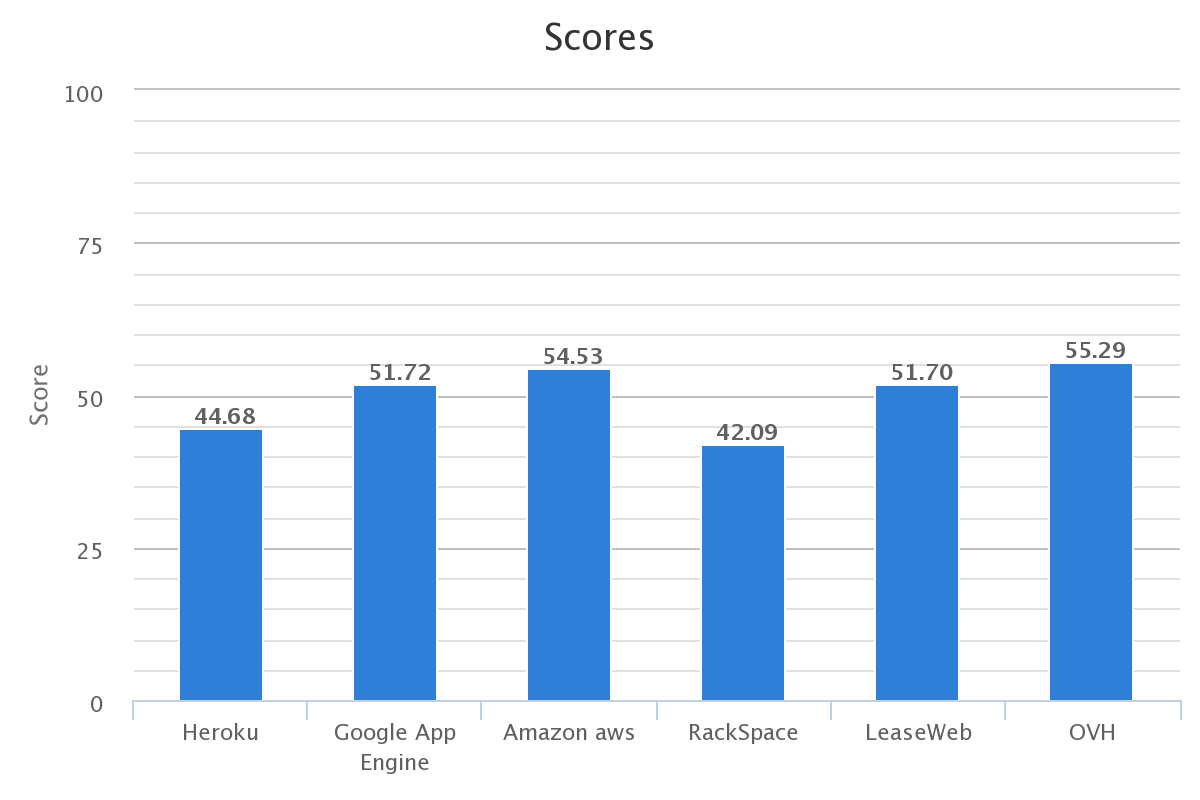
\includegraphics[width=\textwidth-5cm]{img/Result/ranking.png}
  \caption{Ranking.}
  \label{fig:ranking}
\end{figure}

\begin{figure}[h]
  \center
  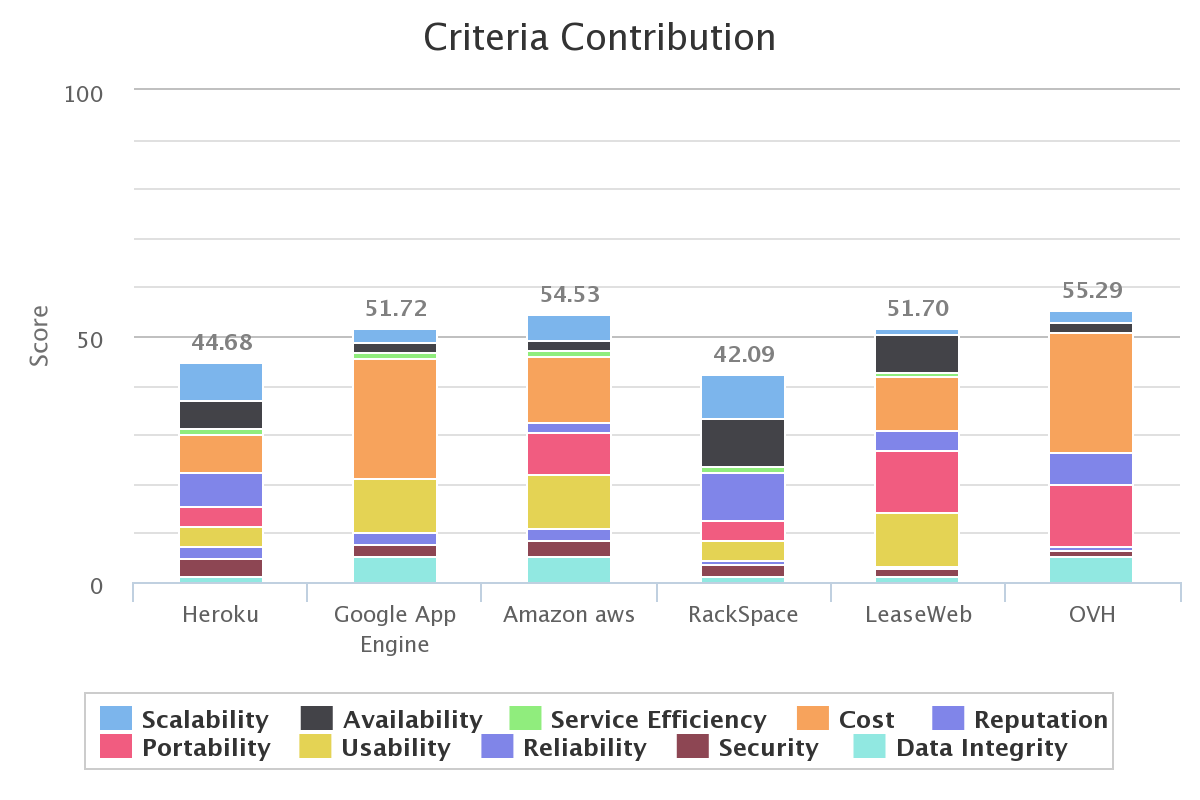
\includegraphics[width=\textwidth-5cm]{img/Result/criteria_contribution.png}
  \caption{Criteria contribution in the final ranking.}
  \label{fig:contrib}
\end{figure}

The graph showed in figure~\ref{fig:spider} is constructed by drawing an axis for each criteria and plotting colored points on the axes. One color correspond to one alternative. The closest a point is to the edge of the figure, the better the corresponding alternative meets the criteria corresponding to this axis.\\

\begin{figure}
\centering
  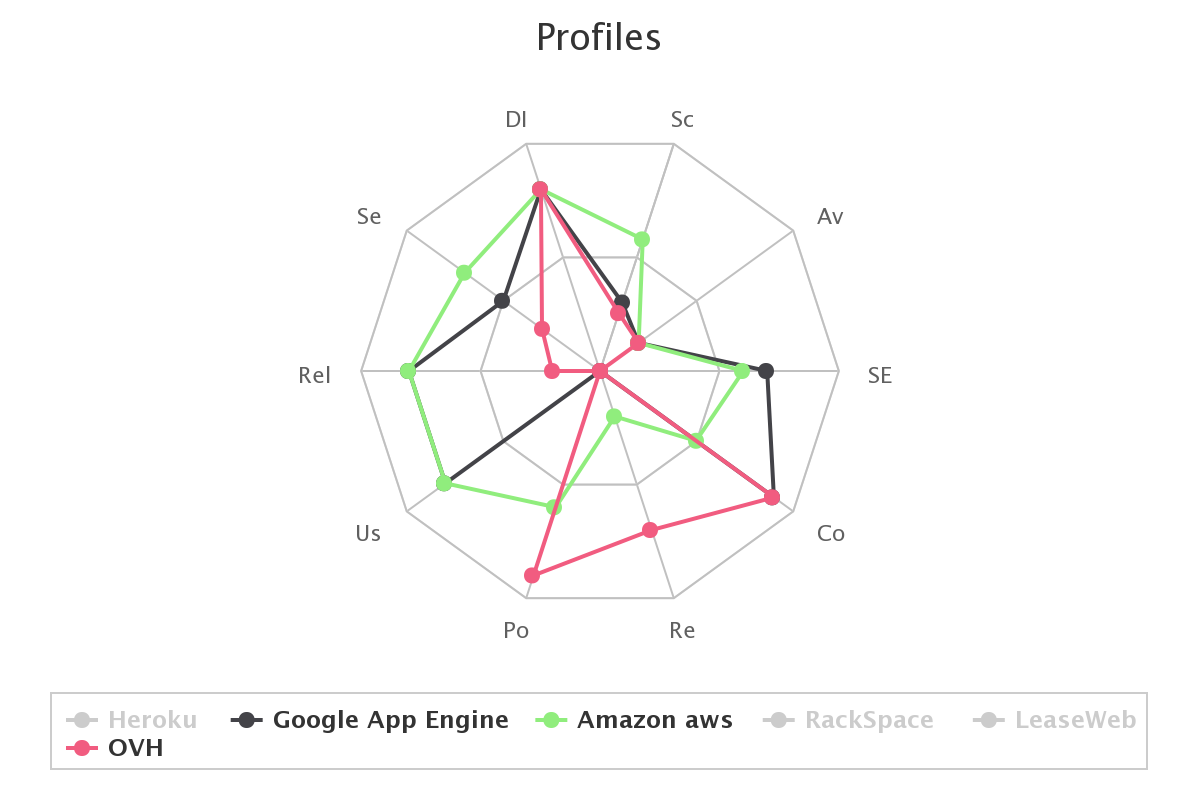
\includegraphics[width=\textwidth-2cm]{img/Result/spider_web-3best.png}
\caption{\og Spider \fg{} representation of the 3 best alternatives.}
  \label{fig:spider}
\end{figure}

\subsection{GAIA Plan}

\begin{figure}
  \centering
  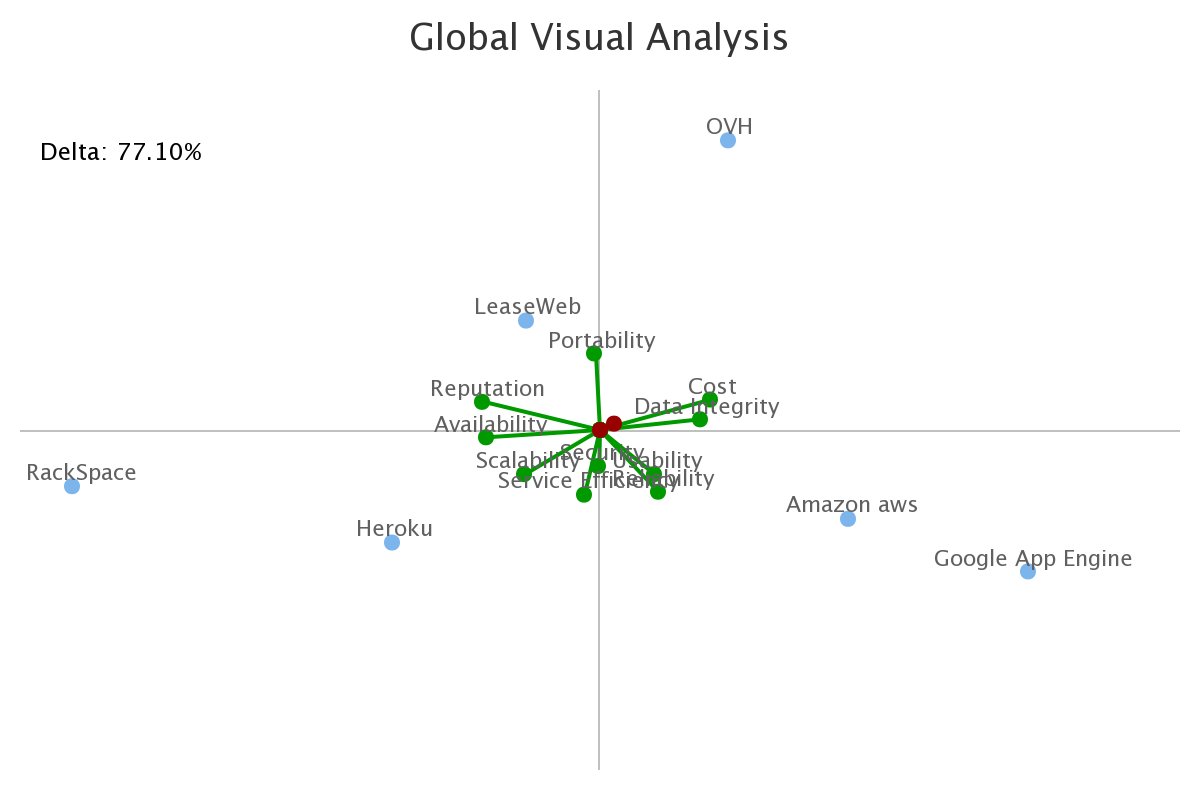
\includegraphics[width=\textwidth-2cm]{img/Result/gaia_plane.png}
  \caption{GAIA representation of the system.}
  \label{fig:gaia}
\end{figure}

The GAIA graph is a great tool to visualize a high dimensional space in a 2-dimensional space. It allows the decision maker to visualize the main characteristics of a decision problem and rapidly see the conflicts or synergies between the criteria as well as strengthen individual alternative performances.

\subsubsection*{Description of the figure \ref{fig:gaia}}

Each green line is a given axis for a criterion. Score for this criterion increases in the direction of the line's dotted end. A score for a given pair of alternative and criteria can be obtained by projecting the point representing the alternative on the criterion's axis. \\

\emph{Important note: } In the upper left corner we see the \textit{Delta} value equal to 77.10\%. This reflect the degree of trust we should give to the graph. Indeed, during the process of dimensionality reduction, information could have been lost. A \textit{Delta} equal to 100\% means that no information has been lost during the process.\\

Here, we can observe that OVH and Google App Engine are similar in term of cost and completely opposed to RackSpace, which feature a good scalability, a great availability and a good reputation but is cost inefficient. \\
We can also clearly see that features (criteria) comes by sacrificing the \emph{cost} criterion. The more a solution is expensive, to better it will score in other criteria.\\
The three most centered alternatives, LeaseWeb, AWS and Heroku have a more average score in all criteria than other alternatives, but we see that AWS seems above this average.\\

\subsection{Stability}

\begin{figure}
  \centering
  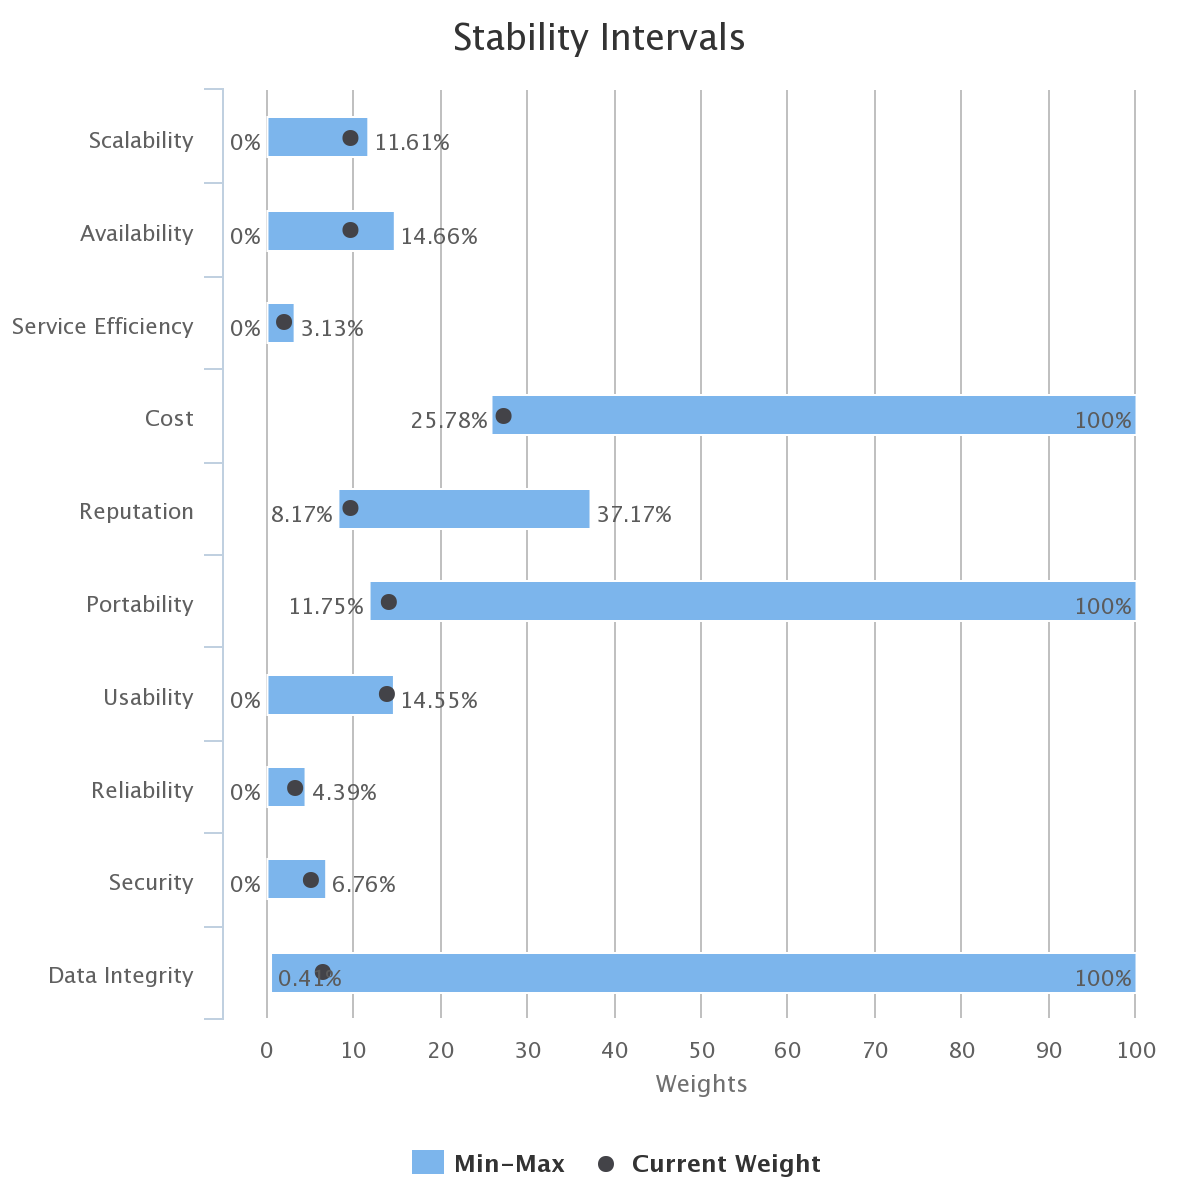
\includegraphics[width=\textwidth-4cm]{img/Result/stability_chart.png}
  \caption{Stability chart for the best alternative (OVH).}
  \label{fig:stab}
\end{figure}

A fundamental part of the analysis resides in finding the stability properties of the ranking. From the analysis of the global ranking as shown above, we can only see that all the alternative are all quite worthy. No alternative seem dominant. But, for example, how does the system react in case of modification of the weights? Does it remain stable and the ranking remain the same, or can the ranking be completely changed or even reversed? That is what will determine now.\\

\subsubsection*{Description of the figure \ref{fig:stab}}

On each row, the black point indicates the current value of the weight of the criteria corresponding to its row. The blue bars indicates the range of value that we could assign to the weight of the corresponding criterion without actually modifying the position of the current best alternative (here : OVH).\\

For example, we see that the current assigned weight for the cost criterion is 27.17\%, but is we would value it lower than 25.78\%, OVH would not remain the best alternative. In contrast, we see that we can value it up to 100\%, OVH would remain the best option, since it is the cheapest.\\

The overall conclusion that we can state after visioning this chart is that the current ranking is very unstable. OVH has very weak dominance over the rest of the alternative in almost all the criteria. A slight modification of any of the weights can cause OVH to loose its current leader position.\\

We can, again, observe that the \textit{data integrity} criterion does not play a crucial role in the final ranking.

\section{Weights Elicitation}

Previously, the weights were assigned by asking a percentage expressing the importance of a criterion. Afterwards, those weights are normalized in order to get a consistent weights assignation. Assigning those weights was not a trivial task because the considered criteria are all of the \emph{quality of service} type and some criterion are predominating then we had to modify the normalized weights to get accord with the Railnova's preferences.\\

Though, we have decided to give a try to the \emph{Weights Elicitation} assignation. Assigning weights using an interactive comparison process helps to express the wanted weights assignation because it allows to give a preference order of the criteria, which was clearly the case for this project.\\

It can be observed at the figure~\ref{fig:alt-ranking} that the Amazon AWS alternative is the best one with this weight assignation. The second ranked alternative is OVH thus, we can observe than those two alternatives, even if not in the same order, are still figuring in the top 2. We can also observe at the figure~\ref{fig:alt-stab} that, the Amazon AWS position is more stable, except for the cost criterion, than when OVH was the best one. 

\begin{figure}
  \center
  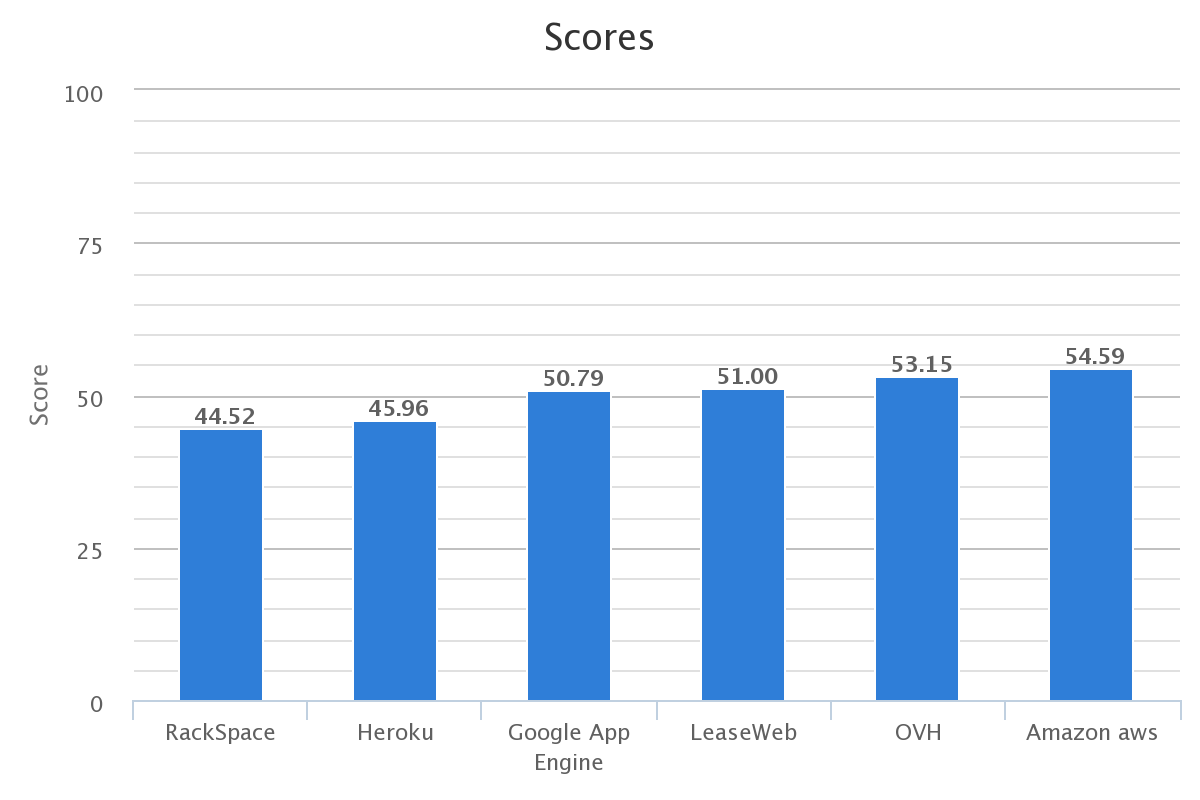
\includegraphics[width=\textwidth-5cm]{img/Result/alternative_ranking.png}
  \caption{Ranking using the weights elicitation feature.}
  \label{fig:alt-ranking}
\end{figure}

\begin{figure}
  \centering
  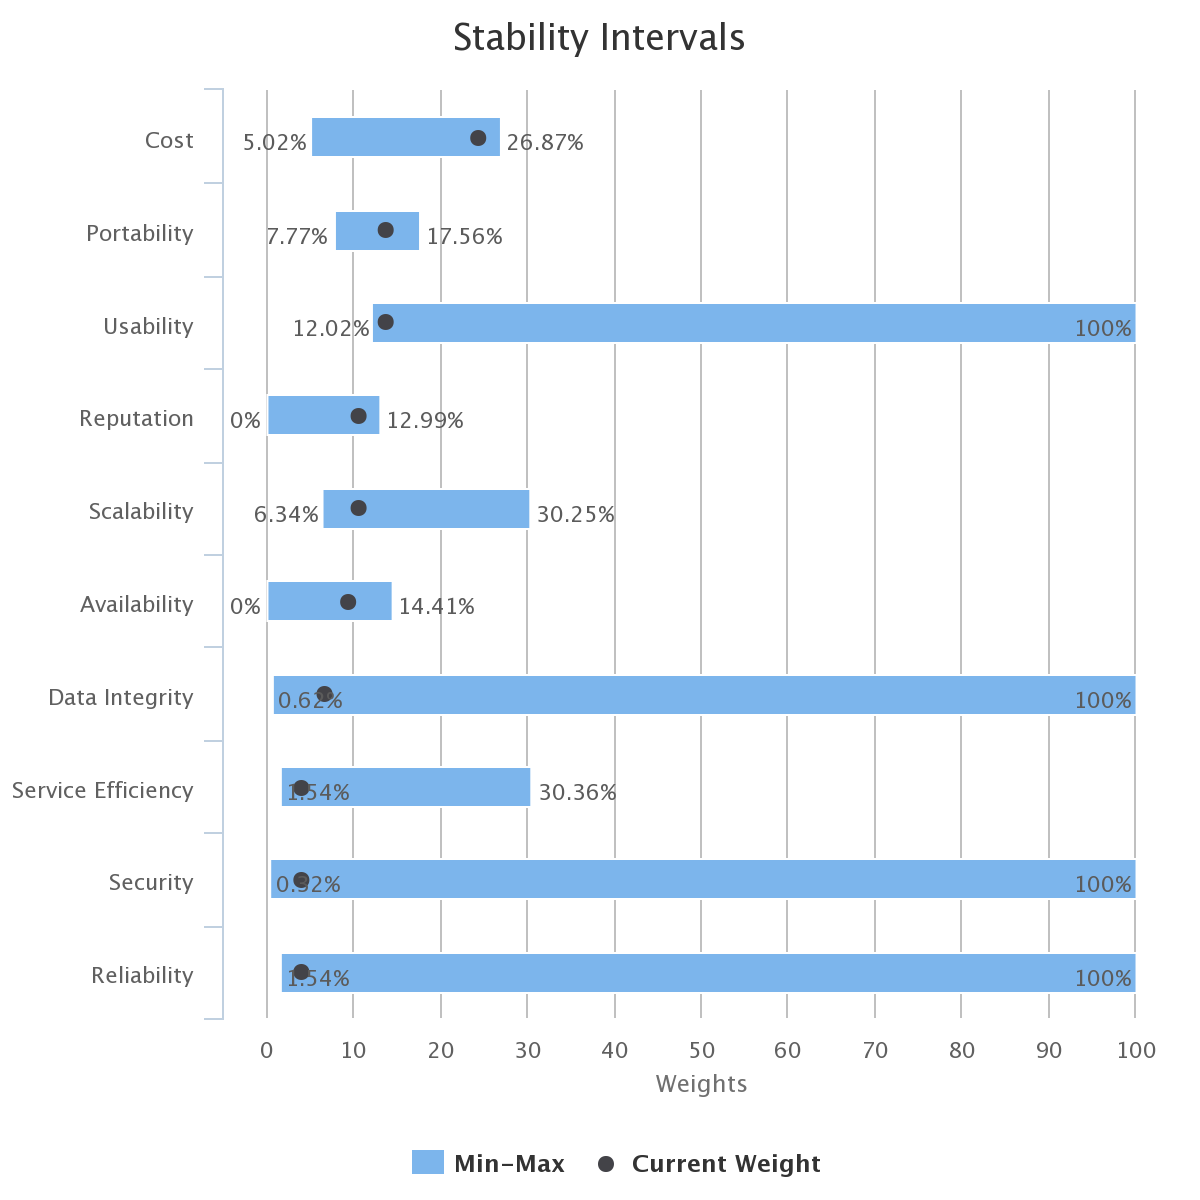
\includegraphics[width=\textwidth-4cm]{img/Result/alternative_stability.png}
  \caption{Stability chart for the best alternative (Amazon AWS) using the weights elicitation feature.}
  \label{fig:alt-stab}
\end{figure}

\section{Conclusion}

Cloud Services providers market is in expansion and is appealing for many developers, start-up companies and big companies. The offers are complex and every cloud provider make the comparison with others harder by using their own terms to describe their product, or cover hidden prices under custom features. This reflects in a final ranking which is highly unstable and sensitive to the decision maker preferences.\\

Study the decision problem through MCDA tools was a good opportunity for Railnova to reconsider its current infrastructure. After determining relevant criteria, researching informations and interacting with Railnova's company, we came up with a system to evaluate. With the help of D-Sight's software, we were able to rank all the alternatives.\\

The resulting analysis showed that any of the alternative clearly outranks its competitors. Given the preferences of the decision maker, we can give a slight advantage to the OVH's and Amazon's IaaS solutions which are respectively cost efficient and averagely good in every criteria. For the PaaS solutions, Google App Engine appeared to be the best alternative.

\end{document}
